%                                                                 aa.dem
% AA vers. 9.1, LaTeX class for Astronomy & Astrophysics
% demonstration file
%                                                       (c) EDP Sciences
%-----------------------------------------------------------------------
%
%\documentclass[referee]{aa} % for a referee version
%\documentclass[onecolumn]{aa} % for a paper on 1 column  
%\documentclass[longauth]{aa} % for the long lists of affiliations 
%\documentclass[letter]{aa} % for the letters 
%\documentclass[bibyear]{aa} % if the references are not structured 
%                              according to the author-year natbib style

%
\documentclass{aa}  

%
\usepackage{graphicx}
%%%%%%%%%%%%%%%%%%%%%%%%%%%%%%%%%%%%%%%%
\usepackage{txfonts}
%%%%%%%%%%%%%%%%%%%%%%%%%%%%%%%%%%%%%%%%
%\usepackage[options]{hyperref}
% To add links in your PDF file, use the package "hyperref"
% with options according to your LaTeX or PDFLaTeX drivers.
\usepackage[colorlinks=true,citecolor=blue,linkcolor=blue]{hyperref}
% To add links in your PDF file, use the package "hyperref"
% with options according to your LaTeX or PDFLaTeX drivers.
%
\usepackage{natbib}
\bibpunct{(}{)}{;}{a}{}{,} % to follow the A&A style
%\usepackage{enumitem}
\usepackage{bm}
\usepackage{upgreek}
\usepackage[dvipsnames]{xcolor}
\usepackage{amsmath}    % Advanced maths commands
%\usepackage{amssymb}
%

\newcommand{\nlens}{20}

\begin{document} 


   \title{Lens models of galaxy--galaxy strong lenses}

   \subtitle{}

   \author{BDLensing team
          \inst{1}
          \and
          C. Ptolemy\inst{2}\fnmsep\thanks{Just to show the usage
          of the elements in the author field}
          }

   \institute{Institute for Astronomy (IfA), University of Vienna,
              T\"urkenschanzstrasse 17, A-1180 Vienna\\
              \email{wuchterl@amok.ast.univie.ac.at}
         \and
             University of Alexandria, Department of Geography, ...\\
             \email{c.ptolemy@hipparch.uheaven.space}
             \thanks{The university of heaven temporarily does not
                     accept e-mails}
             }

   \date{Received September 15, 1996; accepted March 16, 1997}

% \abstract{}{}{}{}{} 
% 5 {} token are mandatory
 
  \abstract
  % context heading (optional)
  % {} leave it empty if necessary  
   {To investigate the physical nature of the `nuc\-leated instability' of
   proto giant planets, the stability of layers
   in static, radiative gas spheres is analysed on the basis of Baker's
   standard one-zone model.}
  % aims heading (mandatory)
   {It is shown that stability
   depends only upon the equations of state, the opacities and the local
   thermodynamic state in the layer. Stability and instability can
   therefore be expressed in the form of stability equations of state
   which are universal for a given composition.}
  % methods heading (mandatory)
   {The stability equations of state are
   calculated for solar composition and are displayed in the domain
   $-14 \leq \lg \rho / \mathrm{[g\, cm^{-3}]} \leq 0 $,
   $ 8.8 \leq \lg e / \mathrm{[erg\, g^{-1}]} \leq 17.7$. These displays
   may be
   used to determine the one-zone stability of layers in stellar
   or planetary structure models by directly reading off the value of
   the stability equations for the thermodynamic state of these layers,
   specified
   by state quantities as density $\rho$, temperature $T$ or
   specific internal energy $e$.
   Regions of instability in the $(\rho,e)$-plane are described
   and related to the underlying microphysical processes.}
  % results heading (mandatory)
   {Vibrational instability is found to be a common phenomenon
   at temperatures lower than the second He ionisation
   zone. The $\kappa$-mechanism is widespread under `cool'
   conditions.}
  % conclusions heading (optional), leave it empty if necessary 
   {}

   \keywords{giant planet formation --
                $\kappa$-mechanism --
                stability of gas spheres
               }

   \maketitle
%
%-------------------------------------------------------------------

\section{Introduction}

Strong gravitational lensing is the phenomenon of forming multiple images from a background source due to the gravitational bending of light path by a massive foreground deflector, such as a galaxy, galaxy group, or cluster. As a result, strong lensing systems are powerful probes of the mass distribution of the foreground deflector \citep[see][for a review on strong lensing by galaxies]{Shajib22}.

Whereas the observed light traces the stars in a lensing galaxy, strong lensing traces the total matter distribution, including dark and baryonic components. As a result, strong lensing can be used to study the relative alignment between dark matter and stars. Any detected offset between these two components can indicate self-interaction in the dark matter particles \citep{Harvey14, Kahlhoefer14, Robertson17}. In the $\Lambda$ cold dark matter ($\Lambda$CDM) cosmology -- the current paradigm to describe our Universe -- the EAGLE simulation predicts no significant offset $\sim$200 pc, regardless of the galaxy being a field galaxy or a cluster member \citep{Schaller15}. Although a recent merger can lead to an offset between the dark matter and stars, these systems are statistically very rare \citep{Schaller15}. On the observational front, only one system has been observed with an offset much larger than this prediction ($1.72\pm 0.42$ kpc), where the deflector consists of two merging galaxies  \citep[][]{Shu16}. %Although there was an initial report of a similar offset for a cluster-member galaxy in Abell 3827 \citep{Williams11, Massey15}, the offset was ruled out with more data \citep{Massey18}.
\citet{Shajib19} find a root-mean-square (RMS) offset in a sample of 13 strong lenses to be 0\farcs04 (i.e., $\sim$200 pc at z$\sim$0.5) excluding three outliers, one of which has two comparable-mass deflectors potentially residing in the same parent halo. Similarly, \citet{Shajib21} constrained a 68 percent upper limit of 218$\pm$19 pc from a sample of 23 galaxy--galaxy lenses.

The misalignment between the mass and light distributions can also be traced using the position angles of the major axes of the elliptical galaxies, which are the most common type of deflectors at the galaxy scale. Previous studies mostly found tight alignment within $\sim$10$\degr$ \citep{Keeton98b, Kochanek02, Treu09, Gavazzi12, Sluse12, Bruderer16, Shajib19, Shajib21}, with higher misalignments are accompanied by large ``external'' shear magnitude, although the vice versa is not necessary. The accompaniment of a large ``external'' shear with a large misalignment can be interpreted as systems in a crowded environment that are not yet dynamically relaxed, as they can have stellar orbits misaligned with the underlying dark matter distribution. Simulations found highly misaligned orbits in isolated systems to be unstable and rare \citep{Heiligman79, Martinet88, Adams07, Debattista15}. However, this interpretation treats ``external'' shear as originating purely from nearby line-of-sight galaxies external to the central deflector. Interestingly, \citet{Etherington23} suggested that this ``external'' shear is not purely of external origin and can arise from the inadequacy of the mass model for lensing galaxy in capturing all of its angular complexity \citep[for example, boxy/discyness, ellipticity gradient, isophotal twists;][]{VandeVyvere22, VandeVyvere22b}. This suggestion from \citet{Etherington23} makes the explanation of high misalignment as stemming from interaction with a crowded environment less favorable.

In this paper, we investigate the alignment between the mass and light using a sample of \nlens\  galaxies. We present power-law mass models of these systems based on \textit{Hubble Space Telescope} (\textit{HST}) imaging data. Using our lens models, we perform two experiments. First, we check if there is a difference in the mass and light offset between isolated and non-isolated galaxies and test the prediction of no difference from the EAGLE simulation. Second, we investigate if the misalignment between light and mass major axes directly correlates with the local galaxy density. This second experiment more directly tests the hypothesis that galaxies with stellar orbits misaligned with dark matter live in crowded environments without adopting the ``external'' shear as a measure of a crowded environment.

This paper is organized as follows. In Section \ref{sec:data}, we describe our lens sample and the \textit{HST} data we model. Then in Section \ref{sec:modeling_method}, we describe our lens modelling method. We present our results in Section \ref{sec:result}. Finally, we discuss our result and conclude the paper in Section \ref{sec:discussion}. Throughout the paper, we adopt a flat $\Lambda$CDM cosmology as the fiducial cosmology with $H_0= 70$ km s$^{-1}$ Mpc$^{-1}$ and $\Omega_{\rm m} = 0.3$.

\section{Data} \label{sec:data}
Our sample comprises of 20 strong lensing systems. All of the strong galaxy-galaxy lensing candidates discovered in the Dark Energy Spectroscopic Instrument (DESI) Legacy Imaging Surveys, Data Release 7, using a deep neural network. Each system in our sample has multiple lensed images. In this section, we first describe the high-resolution imaging data obtained through HST. We then provide a brief overview of the lens systems in the sample.


\subsection{\textit{HST} imaging} 

Images of the lenses were obtained using the HST Wide Field Camera 3 (WFC3) in a specific filter: F140W in the infrared (IR) channel. The wide F140W filter covers the gap between the J and H bands that is inaccessible from the ground. 

% example https://arxiv.org/pdf/2008.11724.pdf and https://arxiv.org/pdf/1807.09278.pdf

\subsection{Description of special systems (can be finalized later)}

% example in https://arxiv.org/pdf/1807.09278.pdf

\begin{figure*}
	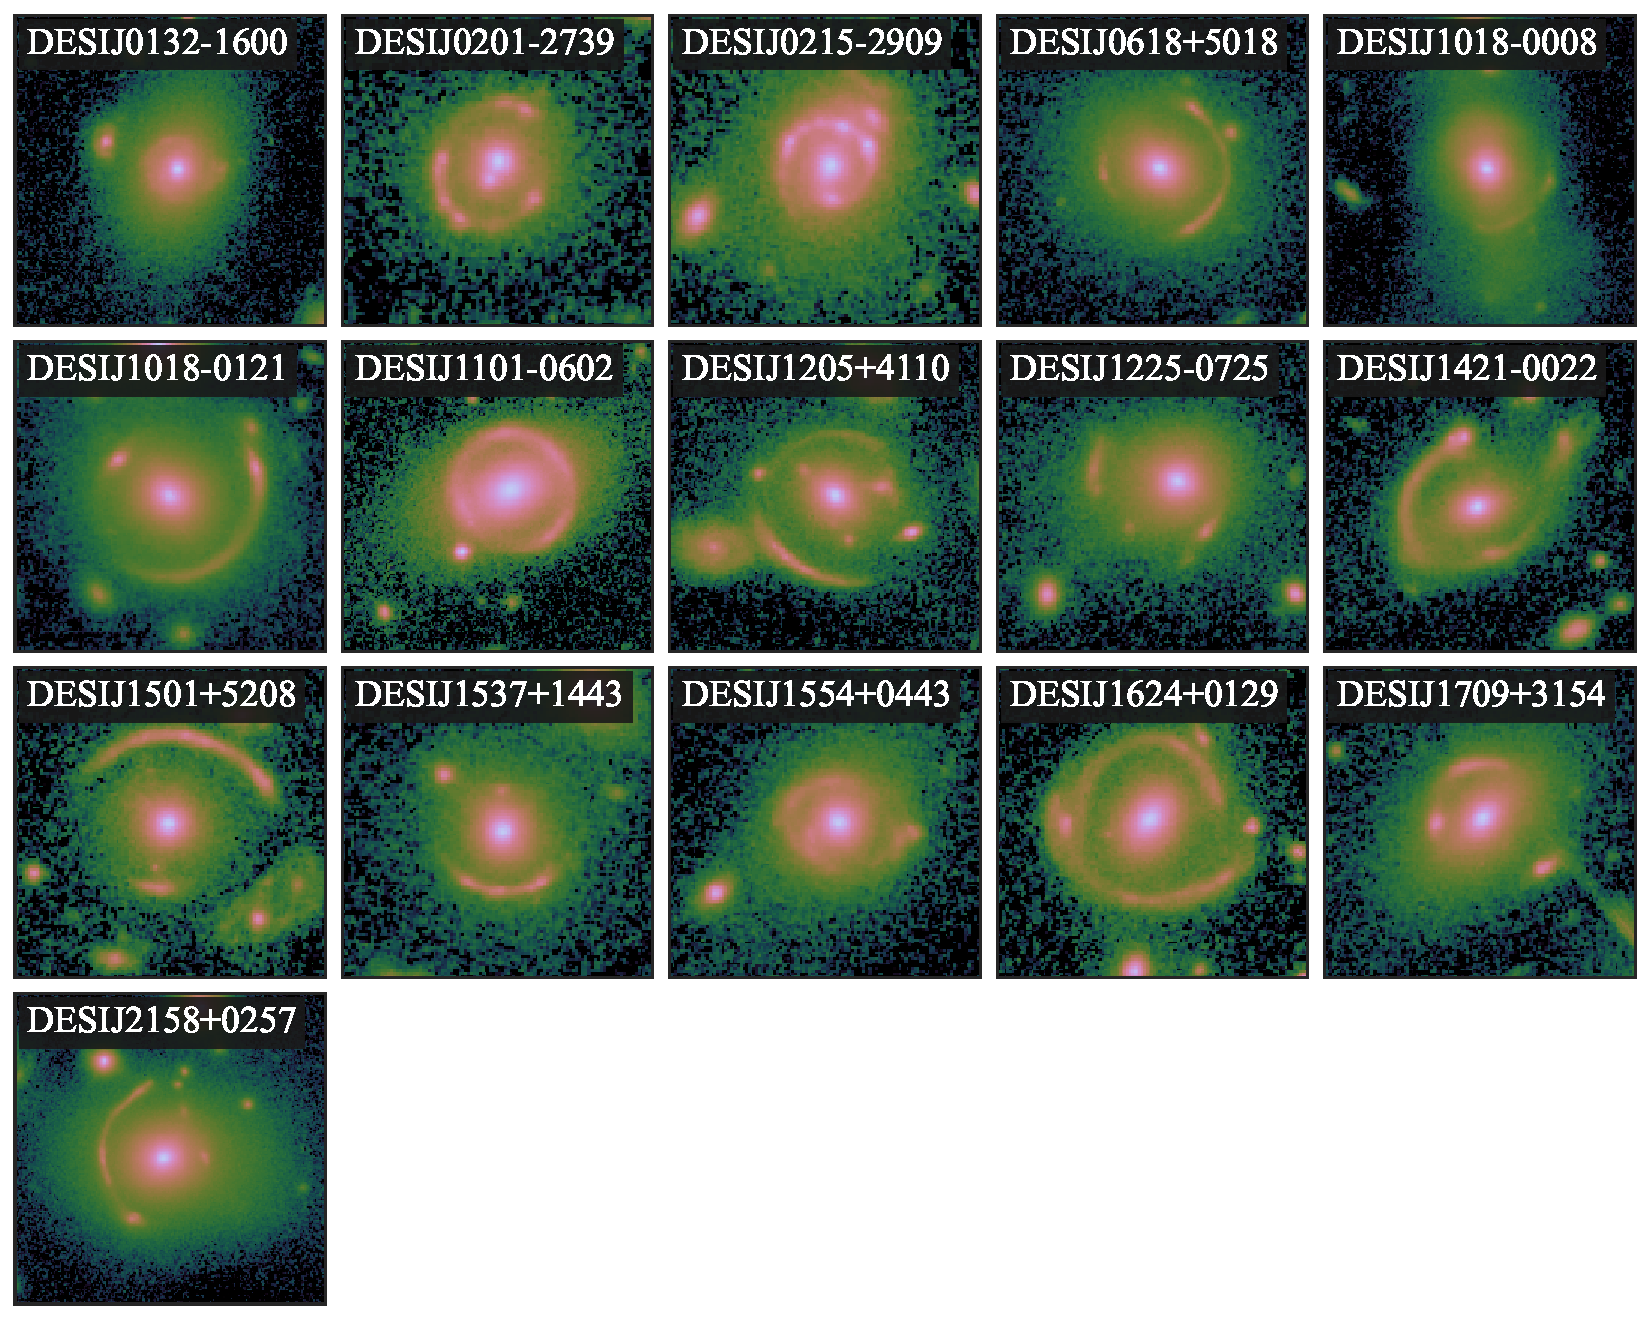
\includegraphics[width=\textwidth]{figures/lens_montage.pdf}
	\caption{\label{fig:montage}
	Montage of all the lens systems.
	}
\end{figure*}

\section{Lens modelling (Method)} \label{sec:modeling_method}

To model the lenses, we used the lens modeling software lenstronomy, available on GitHub1 (Birrer et al. 2015; Bir-rer \& Amara 2018).

\subsection{Lens model ingredients}

\subsubsection{Mass profile}
% EPL, external shear 
% example https://arxiv.org/pdf/1807.09278.pdf
\textbf{EPL:} Elliptical Power Law mass profile is given by, 

$$
\kappa\left(x, y\right)=\frac{3-\gamma}{2}\left(\frac{\theta_{\mathrm{E}}}{\sqrt{q x^2+y^2 / q}}\right)^{\gamma-1}
$$

The Elliptical Power Law (EPL) mass profile represents a specific form of the mass distribution used in gravitational lensing studies. It describes the convergence (\(\kappa\)) in terms of the coordinates \(x\) and \(y\) in an elliptical system, where \(x\) and \(y\) represent the Cartesian coordinates on the lens plane, and \(\theta_{\mathrm{E}}\) is the Einstein radius. The parameter \(q\) denotes the axis ratio of the ellipse, representing the elongation or flattening of the mass distribution.
\\
\newline
\textbf{SIE:} Singular Isothermal Ellipsoid (SIE) is given by,

$$
\kappa\left(x, y\right)=\frac{1}{2}\left(\frac{\theta_{\mathrm{E}}}{\sqrt{q x^2+y^2 / q}}\right)
$$

The factor $\frac{1}{2}$ is introduced to scale the convergence appropriately for the SIE model. We used this profile for the fit of the neighboring satellite galaxies.
\\
\newline
\textbf{Shear:} Shear is a measure of the differential stretching or distortion of the images of background sources due to the gravitational lensing effect. It quantifies how much the shapes of background objects are elongated or deformed by the gravitational field of the lensing mass.\\


The pseudo-vector $\vec{\gamma}$=$(\gamma_1, \gamma_2)$ on the lens plane, whose components are
%
\begin{equation}
    \begin{aligned}
        & \gamma_1(\vec{x})=\frac{1}{2}\left(\Psi_{11}-\Psi_{22}\right) \\
        & \gamma_2(\vec{x})=\Psi_{12}=\Psi_{21},
    \end{aligned}
\end{equation}
%
This is called the shear. The eigenvalues of the shear matrix are
$$
\pm \sqrt{\gamma_1^2+\gamma_2^2}= \pm \gamma \text {. }
$$
Thus, there exists a coordinate rotation by an angle $\phi$ such that
$$
\left(\begin{array}{cc}
\gamma_1 & \gamma_2 \\
\gamma_2 & -\gamma_1
\end{array}\right)=\gamma\left(\begin{array}{cc}
\cos 2 \phi & \sin 2 \phi \\
\sin 2 \phi & \cos 2 \phi
\end{array}\right)
$$
\\
\newline 
\textbf{Flexion:} The second order lensing effect can be expressed in terms of the derivatives of the shear (or in terms of the third derivatives of the potential). We can construct the complex quantities
$$
F= F_1 + iF_2 = \left(\gamma_{\mathrm{1,1}} + \gamma_{\mathrm{2,2}}\right) + i\left(\gamma_{\mathrm{2,1}} - \gamma_{\mathrm{1,2}}\right)
$$
$$
G= G_1 + iG_2 = \left(\gamma_{\mathrm{1,1}} - \gamma_{\mathrm{2,2}}\right) + i\left(\gamma_{\mathrm{2,1}} + \gamma_{\mathrm{1,2}}\right)
$$
which are called first and second flexion, respectively. They describe second order distortions of the images of lensed sources. The flexion is responsible for introducing a curvature and other anisotropic distortions
in the images.


\subsubsection{Light profiles}
% Sersic or double sersic for lens galaxy
% Sersic + shapelets for source galaxy

We chose the elliptical Sersic function (Sersic 1968) to model the deflector light profile. The Sersic profile is parameterized as
$$
I\left(x_1, y_2\right)=I_{\mathrm{e}} \exp \left[-k\left\{\left(\frac{\sqrt{x^2+y^2 / q_{\mathrm{L}}^2}}{\theta_{\mathrm{eff}}}\right)^{1 / n_{\text {Sersic }}}-1\right\}\right] .
$$

where $R_{\rm eff}$ is the effective radius, $I_e$ is the surface brightness at $R_{\rm eff}$, $q_L$ is axis ratio, $n_{\rm Sersic}$ is the Sérsic index, and $k$ is a normalizing constant so that $R_{\rm eff}$ becomes the half-light radius (Sérsic 1968).

\subsection{Modelling procedure}

% description of PSO, MCMC etc.

\section{Result} \label{sec:result}

\subsection{Lens model parameters}

\begin{figure*}
	\centering
	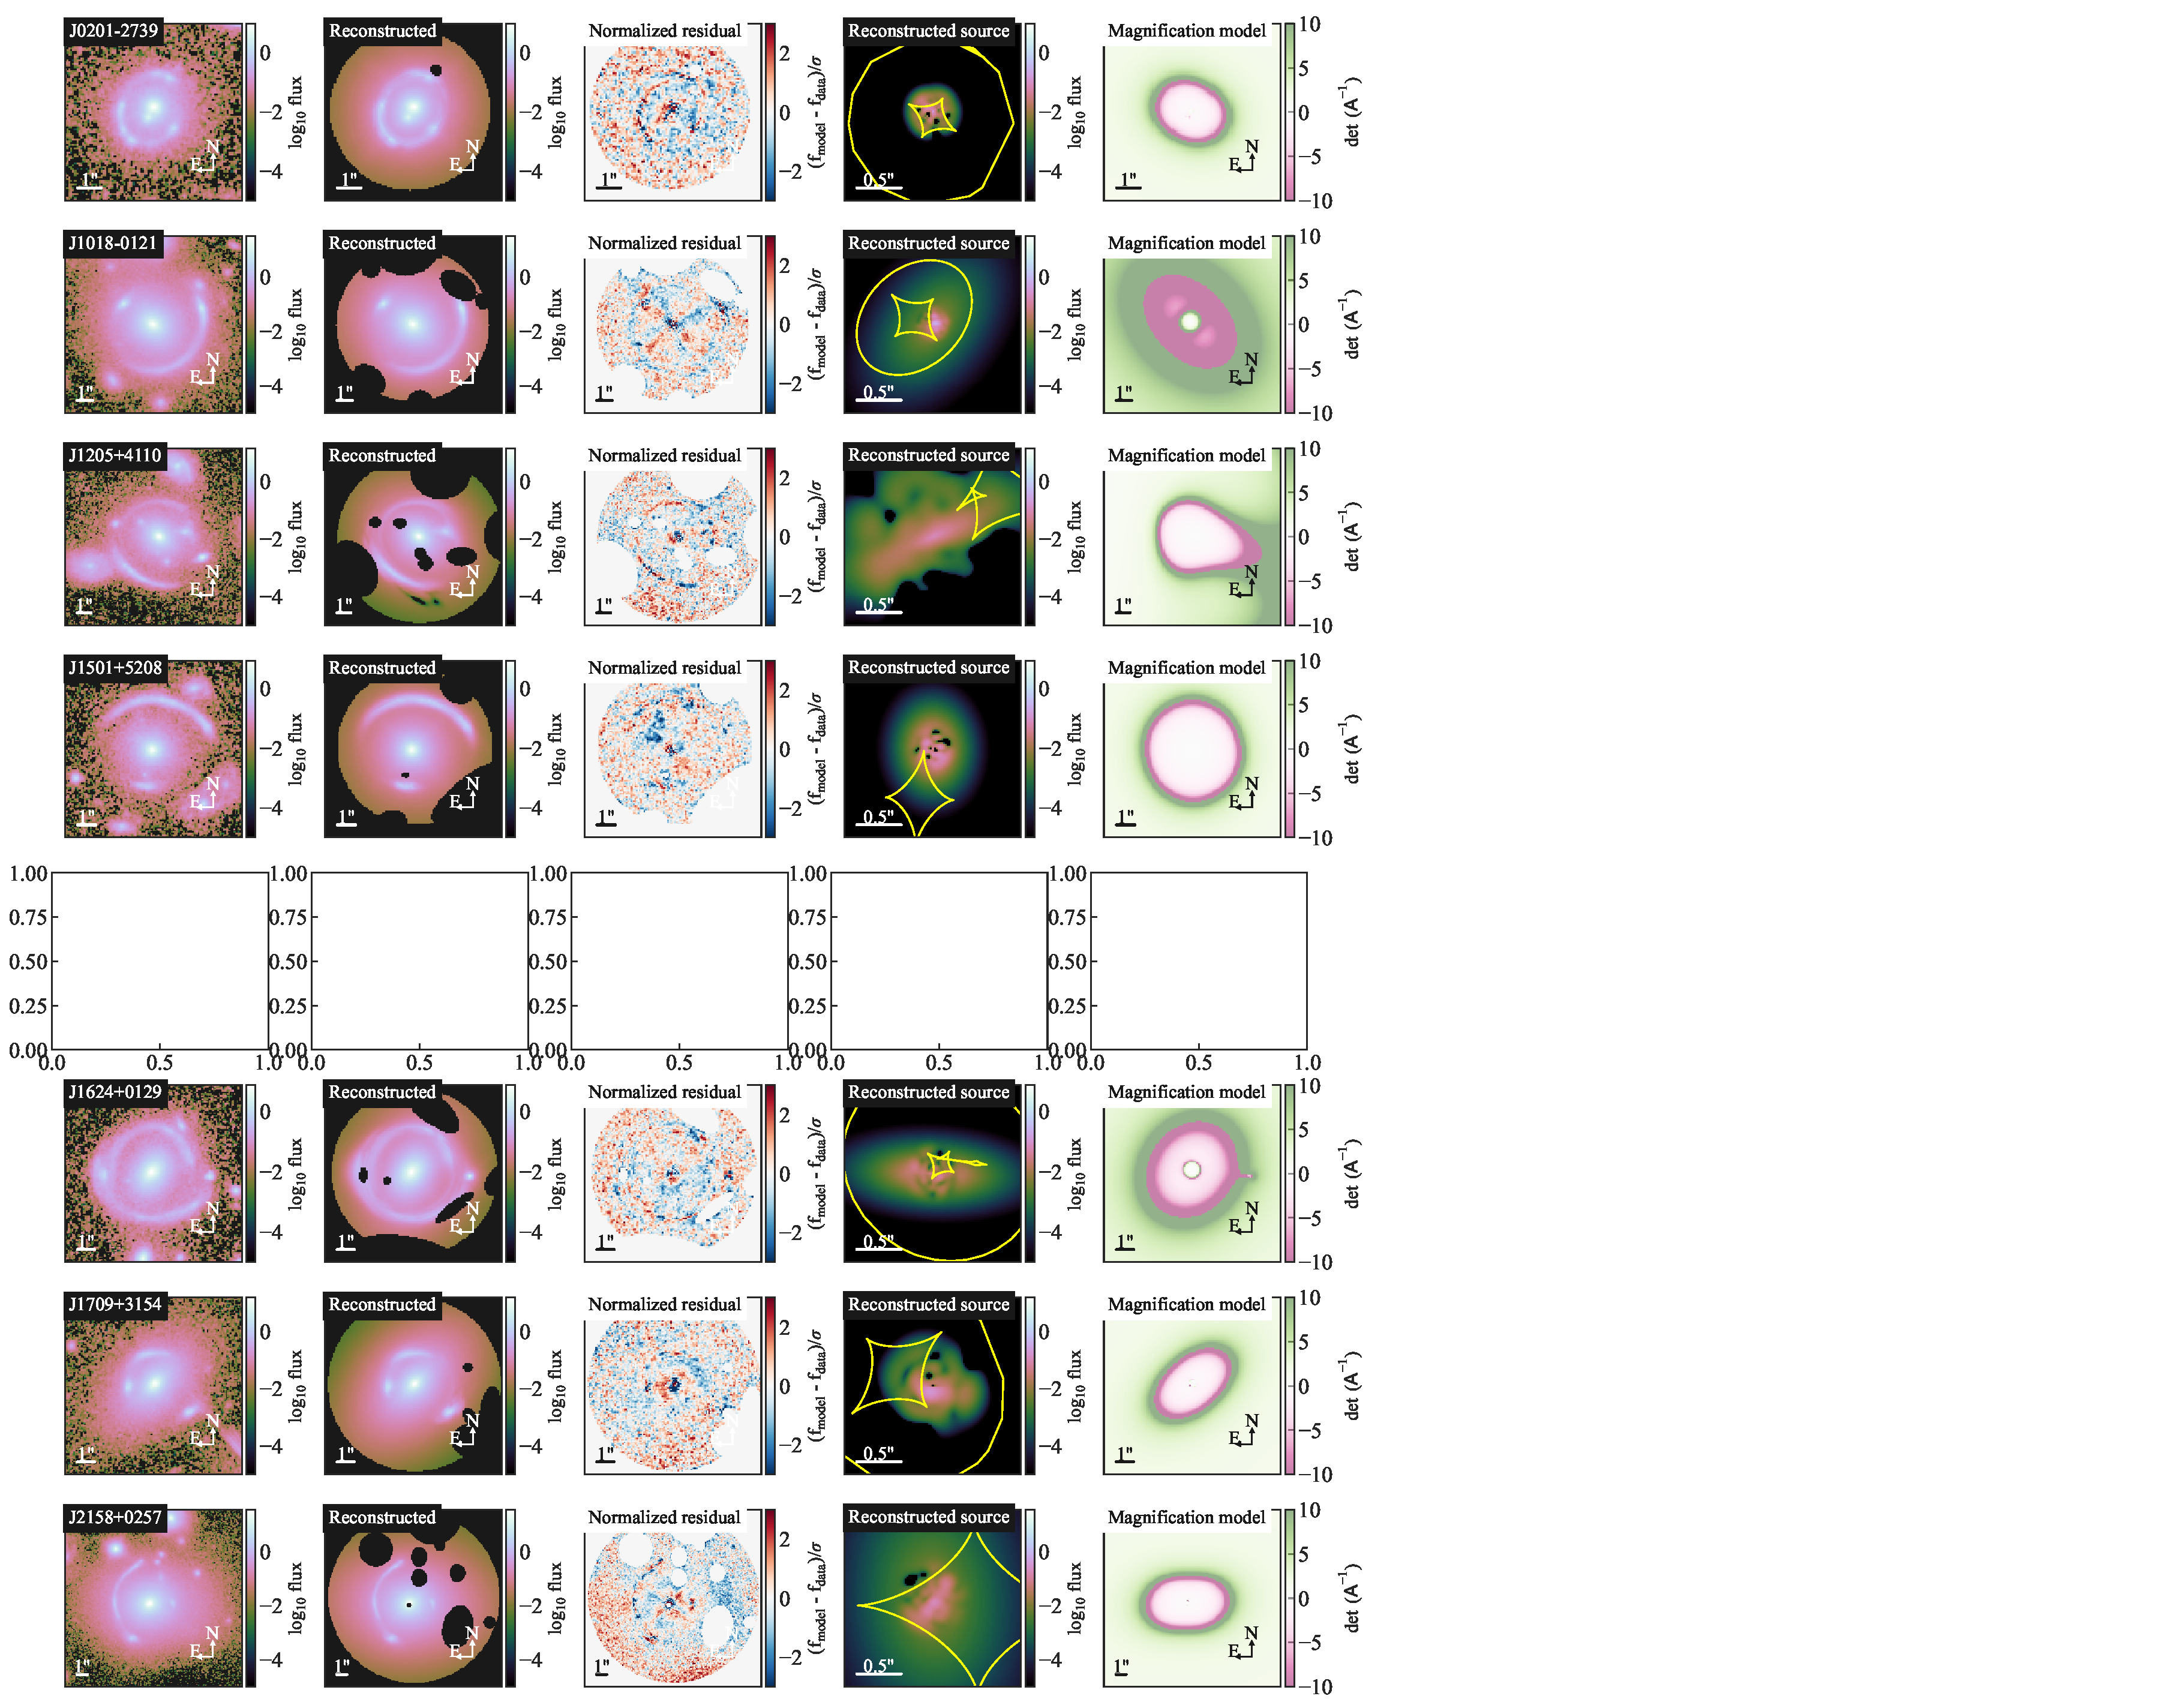
\includegraphics[width=1.55\textwidth]{figures/lens_models.pdf}
	\caption{\label{fig:montage}
	Illustration of the lens models for the lens systems in our sample.
	}
\end{figure*}

 \begin{table*}
 \caption{Lens model parameters: $\theta_{\rm E}$ is the Einstein radius, $\gamma$ is the logarithmic slope of the mass profile, $q_{\rm m}$ is the mass axis ratio, $\phi_{\rm m}$ is the major axis position angle for mass,  $\gamma_{\rm shear}$ is the residual shear magnitude and $\phi_{\rm shear}$ is the residual shear angle,
 $R_{\rm eff}$ is the effective radius of the light profile,  $q_{\rm L}$ is the light axis ratio, and $\phi_{\rm L}$ is the major axis position angle for light. The point estimates are the medians of the 1D marginalized posteriors and the 1$\sigma$ uncertainties are obtained from the 16th and 84th percentiles.
 }
 \label{table:lens_params}
\begin{tabular}{lccccccccc}
\hline
     System &  $\theta_{\rm E}$ &    $\gamma$ &    $q_\text{m}$ &     $\phi_\text{m}$ &  $\gamma_\text{shear}$  &  $\phi_\text{shear}$  &
     $R_{\rm eff} $ & 
     $q_\text{L}$ & 
     $\phi_\text{L}$
     \\
     & (arcsec) & & &(deg, N of E)   & & (deg, N of E) & (arcsec) & & (deg, N of E)\\
\hline
% column values go here
\hline
\end{tabular}
\end{table*}

% need table of model parameters, example https://arxiv.org/pdf/2008.11724.pdf

\subsection{Estimation of $\Sigma_{10}$}



\subsection{Mass and light alignment}

% Pearson correlation coefficient: https://en.wikipedia.org/wiki/Pearson_correlation_coefficient

\section{Discussion and conclusion} \label{sec:discussion}

\begin{acknowledgements}
      Part of this work was supported by the German
      \emph{Deut\-sche For\-schungs\-ge\-mein\-schaft, DFG\/} project
      number Ts~17/2--1.
\end{acknowledgements}

% WARNING
%-------------------------------------------------------------------
% Please note that we have included the references to the file aa.dem in
% order to compile it, but we ask you to:
%
% - use BibTeX with the regular commands:
%   \bibliographystyle{aa} % style aa.bst
%   \bibliography{Yourfile} % your references Yourfile.bib
%
% - join the .bib files when you upload your source files
%-------------------------------------------------------------------

% - use BibTeX with the regular commands:
\bibliographystyle{aa} % style aa.bst
\bibliography{ajshajib} % your references Yourfile.bib

\end{document}